\documentclass[11pt]{article}

\usepackage[margin=1in]{geometry}
\usepackage[T1]{fontenc}
\usepackage[utf8]{inputenc}
\usepackage{lmodern}
\usepackage{microtype}
\usepackage{hyperref}
\usepackage{xcolor}
\usepackage{enumitem}
\usepackage{booktabs}
\usepackage{graphicx}
\usepackage{float}

\hypersetup{
    colorlinks=true,
    linkcolor=blue,
    urlcolor=blue,
    citecolor=blue
}

\setlist[itemize]{leftmargin=1.5em}
\setlist[enumerate]{leftmargin=1.8em}

\newcommand{\course}{CS336 Spring 2026}
\newcommand{\assignment}{Assignment 4: Filtering Language Modeling Data}
\newcommand{\studentname}{Lenard Strahringer}
\newcommand{\sunetid}{lenardst}
\newcommand{\collaborators}{None}

\newcommand{\answer}[1]{#1}

\title{\assignment\\\large Write-Up}
\author{\studentname\\\sunetid}
\date{\today}

\begin{document}
\maketitle


\section{look\_at\_cc}
\subsection*{(a) First WARC page}
\answer{The first page URL is \url{http://020bld.cn.vauofnj.cn/html/991f998999.html}. The hostname does not resolve, so the page is not reachable now. From the translation of the HTML title and metadata, the page is a Chinese article about cleaning lily pollen stains.}

\subsection*{(b) First WET page quality}
\answer{Most of the extracted text is the basic structure of the site: navigation links, contact info, and footer fragments. This text should be filtered out. Training on it would make the model produce template language, not coherent text. The Q\&A section about lily pollen stains is useful.}

\subsection*{(c) Domain usefulness}
\answer{The example is useful for training models on Chinese how-to or FAQ web content. It is not useful for training models on literary fiction.}

\subsection*{(d) 25-record annotation}
\answer{
\begin{enumerate}
    \item \textbf{zho/eng}, \texttt{021sakura.com}: Chinese site index. Mostly navigation text.
    \item \textbf{zho/jpn/eng}, \texttt{044mm.com}: adult video listing. Low value.
    \item \textbf{zho}, \texttt{0553njl.com}: corporate page. Mixed content and template text.
    \item \textbf{zho}, \texttt{0553njl.com}: company news page. Site chrome and updates.
    \item \textbf{zho}, \texttt{07921.cn}: city portal. Heavy navigation and warnings.
    \item \textbf{zho}, \texttt{07921.cn}: job listing. Mostly index text.
    \item \textbf{eng}, \texttt{100.ubc.ca}: UBC biography page. High quality prose.
    \item \textbf{rus/eng}, \texttt{11235813.org}: forum help page. Interface text.
    \item \textbf{rus}, \texttt{123-market.ru}: marketplace page. Sparse and template-heavy.
    \item \textbf{deu/eng}, \texttt{homepagemodules.de}: forum profile. Boilerplate.
    \item \textbf{zho}, \texttt{168ps.com}: video aggregation page. Menu text.
    \item \textbf{zho/eng}, \texttt{198gg.com}: adult index page. Tag text.
    \item \textbf{ell/eng}, \texttt{mysch.gr}: Greek helpdesk page. Navigation labels.
    \item \textbf{eng}, \texttt{whitehorseartshow.com.au}: artwork listing. Catalog text.
    \item \textbf{zho/jpn/eng}, \texttt{223hei.com}: adult page. Low quality.
    \item \textbf{zho}, \texttt{250a.com}: dating platform page. Promotional copy.
    \item \textbf{zho}, \texttt{26888hd3.com}: gambling promo. Marketing boilerplate.
    \item \textbf{eng/fra}, \texttt{agse.fr}: scouting blog post. CMS boilerplate plus some prose.
    \item \textbf{unknown}, \texttt{3344eh.com}: nearly empty page. No value.
    \item \textbf{jpn/eng}, \texttt{377410.com}: tutoring page. Some content.
    \item \textbf{zho}, \texttt{37online.com}: gossip listing. Index text.
    \item \textbf{zho}, \texttt{3iio8u.xyyanglao.com}: corporate landing page. Limited text.
    \item \textbf{zho}, \texttt{4008881886.cn}: company profile. SEO catalog text.
    \item \textbf{zho/eng}, \texttt{431dd.com}: adult video page. Low quality.
    \item \textbf{zho}, \texttt{432149.com}: mixed homepage. Noisy fragment.
\end{enumerate}
The first clearly high-quality page is example 7 (UBC biography). It took 7 examples.
}

\section{extract\_text}
\subsection*{(a) Implementation}
\answer{Implemented in \texttt{cs336\_data/extract\_text.py}.}

\subsection*{(b) Comparison with WET}
\answer{Both extractions recover the main topic text. Both keep some structural content like menus and footers. The WET output is slightly cleaner because Common Crawl applies heuristics after plain HTML to text.}

\section{language\_identification}
\subsection*{(a) Implementation}
\answer{Implemented in \texttt{cs336\_data/language\_id.py}.}

\subsection*{(b) Risks and mitigations}
\answer{Wrong language labels can drop target-language text or keep off-target text. This shifts the training distribution and hurts downstream quality. To reduce this risk, I use a confidence threshold and audit samples. I would track per-language retention over time. For low-confidence cases, I would use a second check or send them to an abstain bucket.}

\subsection*{(c) Manual audit of 20 examples}
\answer{I sampled 20 WET documents and compared predictions with my own labels. Predictions matched the document language in this sample. The English fraction was 8/20 = 40\%. A confidence threshold around 0.7 keeps clearly English pages and drops ambiguous ones.}

\section{mask\_pii}
\subsection*{(a) Email masking}
\answer{Implemented in \texttt{cs336\_data/pii\_masking.py}.}

\subsection*{(b) Phone masking}
\answer{Implemented in \texttt{cs336\_data/pii\_masking.py}.}

\subsection*{(c) IPv4 masking}
\answer{Implemented in \texttt{cs336\_data/pii\_masking.py}.}

\subsection*{(d) Risks and mitigations}
\answer{Naive masking has false positives like product IDs that look like phone numbers. It also has false negatives for international formats and obfuscated patterns. Over-masking can change writing style by inserting many placeholders. To reduce these risks I would use locale-specific rules and allowlists for catalog patterns. I would also run regular human audits and combine regex with a model-based detector.}

\subsection*{(e) Manual audit of 20 masked examples}
\answer{I sampled 20 WET records with at least one replacement. One false positive: a Spanish auto-parts page where BOSCH part number \texttt{0445110299} was masked as a phone number. One false negative: a Chinese page with an 11-digit hotline \texttt{13652918981} not matched by my US regex. Email masking looked good in this sample. IP masking did not occur.}

\section{harmful\_content}
\subsection*{(a) NSFW classifier}
\answer{Implemented in \texttt{cs336\_data/harmful\_content.py}.}

\subsection*{(b) Toxic speech classifier}
\answer{Implemented in \texttt{cs336\_data/harmful\_content.py}.}

\subsection*{(c) Risks and mitigations}
\answer{Naive harmful-content filtering removes useful sensitive text and keeps harmful text in low-resource languages. This biases the training data and creates uneven safety behavior. To reduce these risks, I would tune thresholds per language and per classifier. I would keep an abstain band for borderline scores. I would also audit the kept and removed samples with humans regularly.}

\subsection*{(d) Manual audit of 20 examples}
\answer{I ran both classifiers on 20 WET documents and compared them with my own labels. The models flagged 1/20 (5\%) as harmful. One likely false positive was a Galician economics blog flagged as \texttt{toxic} with score 0.85. I did not see clear NSFW false negatives in this sample. A starting policy is to filter at \texttt{nsfw} score \(\ge 0.8\) and \texttt{toxic} score \(\ge 0.9\).}

\section{gopher\_quality\_filters}
\subsection*{(a) Implementation}
\answer{Implemented in \texttt{cs336\_data/gopher\_quality.py}.}

\subsection*{(b) Manual audit of 20 examples}
\answer{17/20 (85\%) passed the filter. Three rejections looked reasonable: a templated shopping page, a page with many symbolic tokens, and a short German civic page. The German page is a likely false positive because compound words inflated mean word length. Language-agnostic thresholds over-penalize some morphologies.}

\section{quality\_classifier}
\subsection*{(a) Training setup}
\answer{Implemented in \texttt{cs336\_data/quality\_classifier.py}.}

\subsection*{(b) Classification function}
\answer{Implemented in \texttt{cs336\_data/quality\_classifier.py}.}

\section{exact\_deduplication}
\subsection*{Implementation}
\answer{Implemented in \texttt{cs336\_data/exact\_deduplication.py}.}

\section{minhash\_deduplication}
\subsection*{Implementation}
\answer{Implemented in \texttt{cs336\_data/minhash\_deduplication.py}.}

\section{filter\_data}
\subsection*{(a) Pipeline and discard breakdown}
\answer{Implemented in \texttt{scripts/filter\_data.py}. The pipeline in order: (1) English filter (\texttt{en} and score \(\ge 0.7\)), (2) NSFW filter (score \(\ge 0.8\)), (3) toxic filter (score \(\ge 0.9\)), (4) Gopher rules, (5) template-URI rule, (6) repeated-template-line rule, (7) PII masking on kept documents. The run processed 7{,}774{,}382 documents, kept 4{,}944{,}713, and dropped 2{,}829{,}669. Drop reasons: language 87, NSFW 10{,}283, toxic 5{,}771, Gopher 987{,}956, template-URI 306{,}084, template-repetition 1{,}519{,}488.}

\subsection*{(b) Runtime}
\answer{I used 8 workers in parallel on Modal. Outputs were merged from per-shard files. Runtime is dominated by WET parsing and fastText calls and scales with document count.}
\begin{table}[H]
    \centering
    \begin{tabular}{lll}
        \toprule
        Filter step & Input count & Output count \\
        \midrule
        Language filter & 7774382 & 7774295 \\
        NSFW filter & 7774295 & 7764012 \\
        Toxic filter & 7764012 & 7758241 \\
        Gopher quality filter & 7758241 & 6770285 \\
        Template-URI filter & 6770285 & 6464201 \\
        Template-repetition filter & 6464201 & 4944713 \\
        \bottomrule
    \end{tabular}
    \caption{Filter accounting on the full corpus run.}
\end{table}

\section{inspect\_filtered\_data}
\subsection*{(a) Five kept examples}
\answer{(1) \texttt{spectrum.library.concordia.ca}: academic repository page. Useful prose plus some navigation. (2) \texttt{creamteasociety.co.uk}: charity event page. Coherent text but menu-heavy. (3) \texttt{zestycrush.com}: travel web story. Readable prose. (4) \texttt{domries.com}: machinery product page. Short technical text plus catalog structure. (5) \texttt{myescambia.com}: county meetings page. Factual administrative text.}

\subsection*{(b) Five removed examples}
\answer{\texttt{cs-medica.com}, \texttt{aecmag.com}, and \texttt{3rgbled.com} were dropped for repeated template lines. \texttt{cablefax.com/tag/...} was dropped by the template-URI rule. \texttt{wwffl.org/phpBB3/faq.php} was dropped for template repetition. This matches the aggregate counts: only 87 documents were dropped by the language filter, while over 1.5 million were dropped for template repetition.}

\subsection*{(c) Iterations}
\answer{The main opportunity is tighter quality control for template-heavy English commercial and adult pages. A next iteration would strengthen domain and page-type filtering and raise harmful-content strictness for short snippets. Adding cross-document dedup before export would also help.}

\section{tokenize\_data}
\subsection*{Tokenization and dataset size}
\answer{Implemented in \texttt{scripts/tokenize\_data.py}. The dataset contains 5{,}512{,}089{,}641 tokens from 3{,}859{,}975 documents.}

\section{train\_model}
\subsection*{Training and best validation loss}
\answer{I trained a GPT-2-sized model (~430M parameters) on the filtered and tokenized dataset (~5.5B tokens) using 8 B200 GPUs on Modal for 16,384 steps. The training data came from the full pipeline described above: English-filtered Common Crawl WET files, cleaned with language, quality, and harmful-content filters, then tokenized with the GPT-2 tokenizer. The log tail from the Modal run did not capture the periodic validation lines, so I ran a separate evaluation pass (200 iterations) on the saved checkpoint afterward. The estimated validation loss is \textbf{3.854356}.}

\subsection*{Learning curve}
\begin{figure}[H]
    \centering
    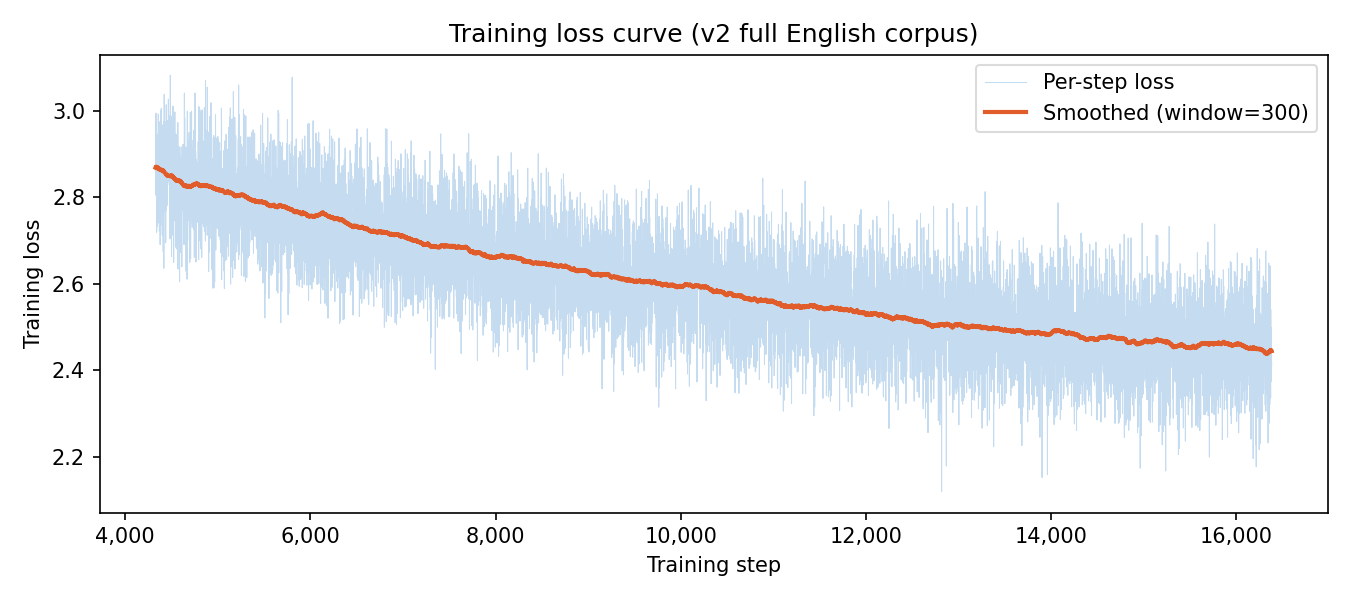
\includegraphics[width=0.85\textwidth]{outputs/filter_data_v2/training_loss_curve_v2.png}
    \caption{Training-loss curve from Modal logs, steps 4328--16383. Earlier steps were not in the captured log tail.}
\end{figure}

\end{document}
